% Group: 	2
% Name: 	Coding Pharaohs
% Document: 	SDD incomplete first draft
% Author:	Matthew Nestor
% Date:		Tuesday September 10 2013

\documentclass[11pt, a4paper,titlepage]{article}
\usepackage[pdftex]{graphicx}
\topmargin -1cm

\begin{document}
 \begin{titlepage}
 \centerline{\small The University of Adelaide}
 \centerline{\small COMP SCI 3006/7015 Software Engineering and Project}
 \vspace{5cm}
 \centerline{\bf \huge Software Design Document}
 \centerline{\bf \huge (SDD)}
 \vspace{0.5cm}
 \centerline{\LARGE for}
 \vspace{0.5cm}
 \centerline{\bf \huge Road Closure Marking}
 \centerline{\bf \huge Robot}
 \vspace{1cm}
 \centerline{Version 0.1}
 \vspace{1cm}
 \centerline{Prepared by Group 2}
  \end{titlepage}
 \tableofcontents
 \newpage
 {\bf \large Change History}\newline

 \begin{tabular}{| c | c | l |}
  \hline
  Date & Version & Reason for Change \\
  \hline
  10th Sept & 0.1 & Initial draft \\
  \hline
 \end{tabular}

 \newpage
  \section{Introduction}
    \subsection{Purpose}
    \subsection{Scope}
    \subsection{References}
    \subsection{Overview}
    \subsection{Constraints}
     \vspace{3cm}

 
  \section{System Overview}
   \vspace{3cm}

  \section{System Architecture and Components Design}
    \subsection{Architectural Description}
    \begin{itemize}
     \item Architectural Pattern: Pipe and Filter
     \item Control Style: Centralised (Manager Model)
    \end{itemize}

    \subsection{Component Decomposition Description}
    \begin{itemize}
     \item Object Oriented Style
    \end{itemize}
    
    \subsection{Detailed Components Design Description}
    \subsection{Architectural Alternatives}
    \subsection{Design Rationale}
    
  \newpage
  \section{Data Design}
    \subsection{Database Description}
    \subsection{Data Structures}
  
  \newpage
  \section{Design Details}
    \subsection{Class Diagrams}
    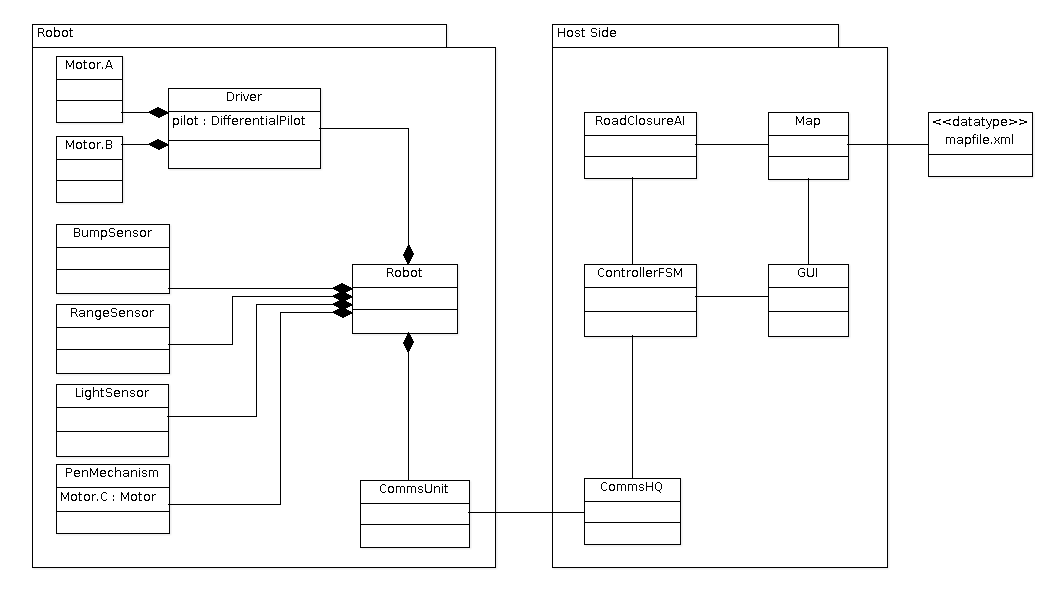
\includegraphics[height=10cm,width=20cm,angle=90]{UML/softwareArch.png}
    \subsection{State Diagrams}
    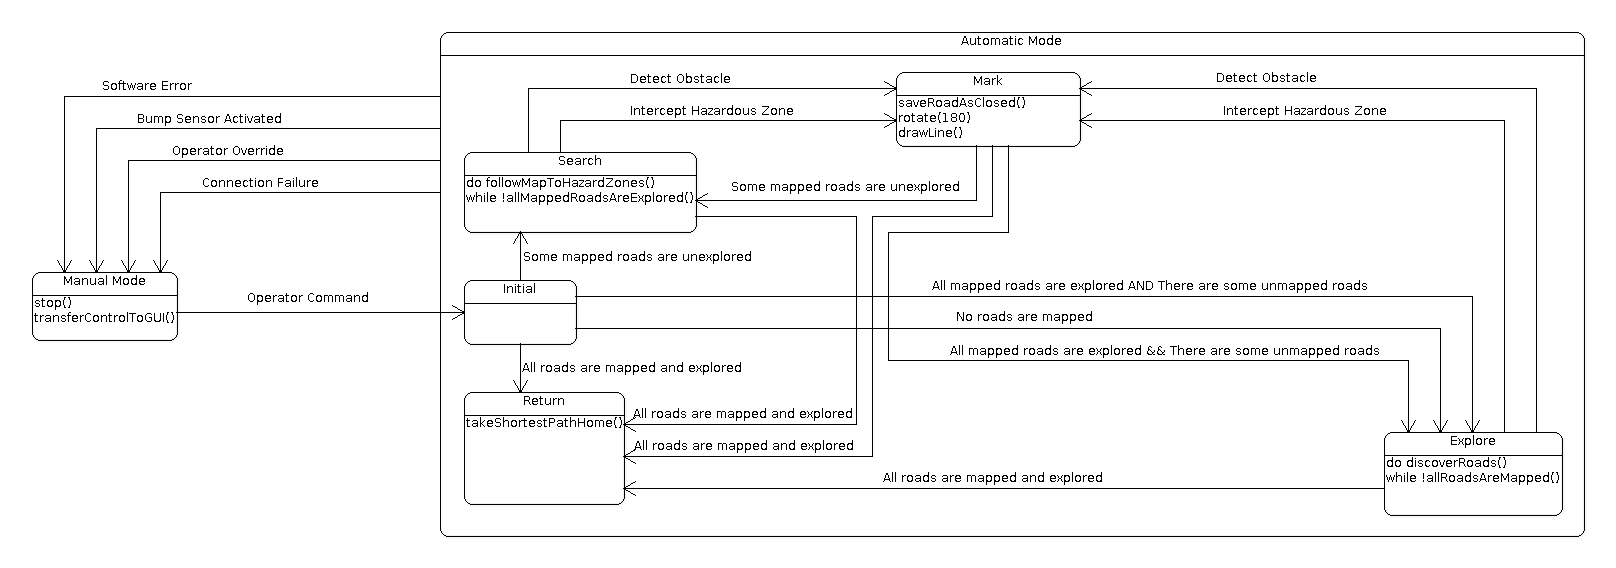
\includegraphics[height=10cm,width=25cm,angle=90]{UML/softwareFSM.png}
    \subsection{Interaction Diagrams}
  
  \newpage
  \section{Human Interface Design}
    \subsection{Overview of the User Interface}
    \subsection{Detailed Design of the User Interface}
    
  \newpage
  \section{Resource Estimates}
   \vspace{3cm}
  \section{Definitions, Acronymns and Abbreviations}
  
\end{document}
